%!TEX root = ../thesis.tex
%*******************************************************************************
%****************************** Third Chapter **********************************
%*******************************************************************************
\chapter{Topology of the Lattice}

% **************************** Define Graphics Path **************************
\ifpdf
    \graphicspath{{Chapter3/Figs/Raster/}{Chapter3/Figs/PDF/}{Chapter3/Figs/}}
\else
    \graphicspath{{Chapter3/Figs/Vector/}{Chapter3/Figs/}}
\fi
QCD presents two properties that distinguish it from the other forces of nature: confinement and dynamical chiral symmetry breaking. Both these properties have been experimentally observed, however a unified theoretical understanding of how they arise from the current standard model of QCD is still a subject of interest.
\section{Confinement}\label{sec:Confinement}
The confinement property of QCD, and the accompanying notion of asymptotic freedom, is one of the defining low-energy features of the theory of the strong interaction. With Gell-mann and Zweig's concurrent proposal of quarks as the elementary constituents of baryons and mesons~\cite{GellMann:1964nj,Zweig:1964jf}, it is natural to then attempt to observe these new particles in isolation. However, efforts to observe quarks proved impossible. Early experiments testing the behaviour of electron-proton collisions demonstrated that protons scatter elastically, behaving as though they are finite-sized particles recoiling electromagnetically from the incident electron~\cite{Hofstadter:1956qs}. These experiments indicated no further substructure to the proton, inconsistent with the quark model. As accelerator energies improved, later experiments~\cite{Bloom:1969kc, Breidenbach:1969kd}, using electron energies of $7$ and $10~\si{GeV}$ found that inelastic scattering effects became dominant, with electrons behaving as though they were scattering off of loosely bound constituent particles. To explain this behaviour, Feynman proposed what is known as the 'parton' model~\cite{Feynman:1969ej}, treating the proton as being comprised of non-interacting electrically charged particles in the limit that the incident electron energy tends towards infinity. This is precisely the notion of asymptotic freedom; at large distance scales the partons are tightly bound, whereas at short distances they behave as free particles. It did not take long for the separate theories of quarks and partons to recognised as complementary, and by the early 70's the quark-parton model of hadrons accurately explained the the experimental results observed in particle colliders.\\

These experimental and theoretical results led in part to the development of the non-Abelian gauge field theory of QCD, as introduced in Chapter~\ref{chapter:LatticeQCD}. The proof that non-Abelian gauge theories are asymptotically free was discovered in 1973~\cite{Gross:1973id}, and experimental evidence of the existence of 3 quark colours through study of the cross section of $e^+ e^-$ collisions supports the initial $SU(3)$ colour symmetry anticipated by Gell-Mann and Zweig. At high energies, QCD has consistently explained the behaviour of hadronic matter, and has become the accepted theory of the strong nuclear interaction. However, the question of whether QCD is indeed a confining theory still remains. As confinement is a low-momentum property of QCD, it is apparent that any analytic proof of confinement must take place far from the asymptotic limit. To date, no such analytic proof has been found.\\

Lattice calculations are currently the only method by which it is possible to investigate low-energy QCD phenomena from first-principles. Calculations of the static potential between two massive quarks, both recent and old~\cite{Born:1993cq, Bonnet:1999gt, Creutz:1980hb, DiGiacomo:1990hc}, have shown that the potential rises linearly at sufficiently large separation distances. This behaviour is precisely what is expected of a colour confining theory. Other confinement mechanisms have also been proposed on the lattice, including mechanisms based on the behaviour of the gluon propagator at $q=0$~\cite{Zwanziger:1991gz} and the behaviour of the pion mass and Polyakov loop at light quark masses~\cite{Iwasaki:1991mr}. All lattice results so far have indicated that QCD is in fact a confining theory at low energy.\\

There is good evidence that confinement has its roots in the topological properties of the QCD vacuum. It is well understood that the QCD vacuum, unlike the QED vacuum, admits non-trivial instanton solutions: solutions of the vacuum field configurations that are all minima of the classical action, yet are distinguished from one another by a topological quantum number~\cite{Belavin:1975fg}. The presence of instanton solutions was significant in resolving the $U(1)$ anomaly~\cite{tHooft:1986ooh}, and provides an excellent method of calculating the ground state hadron spectrum~\cite{Schafer:1996wv}. The non-trivial topology of the QCD vacuum, and the success of topological features in resolving QCD anomalies, motivates the search for a topological explanation of confinement. A variety of features have been proposed, including: Abelian monopoles~\cite{Ivanenko:1990xu, Chernodub:1995tt}, merons~\cite{Callan:1977qs} and dual superconductors~\cite{Mandelstam:1974pi,tHooft:1982ylj}. One of the most promising models in recent years is known as the \textit{Centre Vortex Model}, and it is this model that forms the backbone of this research.
\section{Centre Vortices}
Originally proposed by 't Hooft in 1978~\cite{'tHooft:1977hy,'tHooft:1979uj}, centre vortices are closed two-dimensional surfaces present in four-dimensional Euclidean space. The key property of a centre vortex is that in three dimensions, where the vortices appear as tubes, any Wilson loop (see Sec.~\ref{sec:LatticeDiscretisation}) that encloses a vortex will acquire a centre phase, such that
%
\begin{equation}
W(C)\rightarrow z \,W(C)\, ,
\end{equation}
%
where $z$ is an element of $Z(3)$, the centre of $SU(3)$. The centre of a group is the subgroup that contains all the elements of the group that commute with all other elements. In the case of $SU(3)$ this corresponds to
%
\begin{equation}
Z(3) = \big\lbrace \exp\left(\frac{m\pi i}{3} \right)I ~ | ~ m = 0,\pm 1\big\rbrace\, . 
\end{equation}
%
When considering the value of any given Wilson loop, the centre vortex model suggests that
%
\begin{equation}
W(C) = \prod_i z_i\times \lbrace\text{short-distance physics}\rbrace\, ,
\end{equation}
%
where the $z_i$ correspond to the phases of the centre vortices intersecting the loop $C$. A simple visualisation of this idea is shown in Fig.~\ref{fig:CentreVortex}. It is not immediately apparent why this form of the Wilson loop is related to confinement, however a simple $SU(2)$ calculation motivates the relevance of this model~\cite{Greensite:2016pfc}. To understand the significance of this calculation it is worth first deviating slightly to detail the relationship between the Wilson loop and the potential energy between two massive (static) quarks.\\
% 
\begin{figure}
\centering
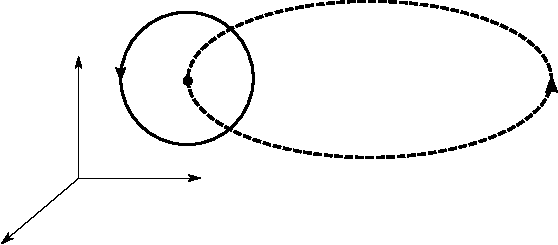
\includegraphics[width=\linewidth]{./centre_vortex.pdf}
\caption{\label{fig:CentreVortex} A single centre vortex (dashed line) intersecting a Wilson loop (solid line) in 3 dimensions. The Wilson loop will acquire a centre phase corresponding to the phase of the vortex.}
\end{figure}
%

Follwing the argument presented in Ref.~\cite{Makeenko:2009dw}, consider a Wilson loop calculated around a rectangle in the $x-t$ plane with dimensions $R\times T$. As the Wilson loop is gauge invariant, we are free to select a convenient gauge in which to perform the calculation. To this end, we choose the fields to be in axial gauge, such that $A_0(x)=0\implies U_0(x) = 1\,\forall\,x$. So the Wilson loop becomes
%
\begin{equation}
W(R\times T) = \Tr \left(U_1(0)\,U_1^\dagger(T)\right)\, .
\end{equation}
%
We can insert a complete set of energy eigenstates, $\sum_n |\,n\rangle\,\langle n \,|=1$ to obtain
%
\begin{align*}
W(R\times T) &= \Tr \left( \sum_n \langle U_1(0)\, |\, n\rangle\,\langle n\, |\, e^{-E_n(R)\, T}\, | \, U_1(0) \rangle\right)\\
&=  \sum_n \Tr \left( \big|\langle U_1(0)\, |\, n\rangle\big|^2 \right)\,e^{-E_n(R)\,T} 
\end{align*}
%
As $T\rightarrow \infty$, the only surviving contribution will be the lowest energy, $E_0(R)$. This means that
%
\begin{equation}
\lim_{T\rightarrow \infty} W(R\times T) \propto e^{-E_0(R)\, T}\, .
\label{eq:WilsonEnergy}
\end{equation}
\\%

With Eq.~\ref{eq:WilsonEnergy} in mind, we return to the aforementioned $SU(2)$ confinement model. Consider a two-dimensional plane with area $L^2$, with $N$ vortices piercing the plane. Then the vortex density $\rho = \frac{N}{L^2}$. The probability of finding $n$ vortex in some region of the plane $A$ is equal to the probability that at least $n$ vortices are in $A$, multiplied by the probability that at least $N-n$ vortices are outside of $A$. Expressed mathematically, this is
%
\begin{equation}
P_N(n) = {N\choose n} \left(\frac{A}{L^2}\right)^n \left(1-\frac{A}{L^2}\right)^{N-n}\, .
\end{equation}
%
In $SU(2)$ the group centre is simply $Z(2) = \pm I$, so the vortices each contribute a phase of $-1$. So the expectation value of the Wilson loop around the perimeter of $A$ takes the value
%
\begin{align}
\langle W(\partial A) \rangle &= \sum_{n=0}^N (-1)^n\,P_N(n)\\
&= \left(1-\frac{A}{L^2}\right)^N\,\sum_{n=0}^N {N\choose n} \left( -\frac{A}{L^2}\left(1-\frac{A}{L^2}\right)^{-1}\right)^n \label{eq:BinomialSum}
\end{align}
%
Making use of the binomial theorem to evaluate the sum in Eq.~\ref{eq:BinomialSum}, we find
%
\begin{equation}
\langle W(\partial A) \rangle = \left(1-\frac{2A}{L^2}\right)^N\, . \label{eq:WilsonFiniteArea}
\end{equation}
%
We then re-express Eq.~\ref{eq:WilsonFiniteArea} in terms of the vortex density $\rho$
%
\begin{equation}
\langle W(\partial A) \rangle = \left(1-\frac{2\rho A}{N}\right)^N\, ,
\end{equation}
%
and take the limit as $L^2,N\rightarrow \infty$ whilst keeping $\rho$ constant to obtain the final result
%
\begin{equation}
\lim_{N\rightarrow \infty} \langle W(\partial A) \rangle = \exp(-2\rho A)\, .
\label{eq:AreaLawFalloff}
\end{equation}
%
Taking $A = R\times T$, we see that from Eq.~\ref{eq:WilsonEnergy}, Eq.~\ref{eq:AreaLawFalloff} implies that $E_0 = 2\rho \,R$. Hence, the potential energy between two massive, static quarks increases linearly with the distance $R$ separating them, which is precisely the confinement scenario!\\

It is important to highlight the assumptions and simplifications made in the above argument. Firstly, this 

\section{Locating Vortices}
\subsection{Maximal Centre Gauge}\label{sec:MCG}
\subsection{Centre Projection}
\section{Instantons}
\subsection{Topological Charge}

%A frequently seen mistake is to use `\textbackslash begin\{center\}' \dots `\textbackslash end\{center\}' inside a figure or table environment. This center environment can cause additional vertical space. If you want to avoid that just use `\textbackslash centering'
%
%
%\begin{table}
%\caption{A badly formatted table}
%\centering
%\label{table:bad_table}
%\begin{tabular}{|l|c|c|c|c|}
%\hline 
%& \multicolumn{2}{c}{Species I} & \multicolumn{2}{c|}{Species II} \\ 
%\hline
%Dental measurement  & mean & SD  & mean & SD  \\ \hline 
%\hline
%I1MD & 6.23 & 0.91 & 5.2  & 0.7  \\
%\hline 
%I1LL & 7.48 & 0.56 & 8.7  & 0.71 \\
%\hline 
%I2MD & 3.99 & 0.63 & 4.22 & 0.54 \\
%\hline 
%I2LL & 6.81 & 0.02 & 6.66 & 0.01 \\
%\hline 
%CMD & 13.47 & 0.09 & 10.55 & 0.05 \\
%\hline 
%CBL & 11.88 & 0.05 & 13.11 & 0.04\\ 
%\hline 
%\end{tabular}
%\end{table}
%
%\begin{table}
%\caption{A nice looking table}
%\centering
%\label{table:nice_table}
%\begin{tabular}{l c c c c}
%\hline 
%\multirow{2}{*}{Dental measurement} & \multicolumn{2}{c}{Species I} & \multicolumn{2}{c}{Species II} \\ 
%\cline{2-5}
%  & mean & SD  & mean & SD  \\ 
%\hline
%I1MD & 6.23 & 0.91 & 5.2  & 0.7  \\
%
%I1LL & 7.48 & 0.56 & 8.7  & 0.71 \\
%
%I2MD & 3.99 & 0.63 & 4.22 & 0.54 \\
%
%I2LL & 6.81 & 0.02 & 6.66 & 0.01 \\
%
%CMD & 13.47 & 0.09 & 10.55 & 0.05 \\
%
%CBL & 11.88 & 0.05 & 13.11 & 0.04\\ 
%\hline 
%\end{tabular}
%\end{table}
%
%
%\begin{table}
%\caption{Even better looking table using booktabs}
%\centering
%\label{table:good_table}
%\begin{tabular}{l c c c c}
%\toprule
%\multirow{2}{*}{Dental measurement} & \multicolumn{2}{c}{Species I} & \multicolumn{2}{c}{Species II} \\ 
%\cmidrule{2-5}
%  & mean & SD  & mean & SD  \\ 
%\midrule
%I1MD & 6.23 & 0.91 & 5.2  & 0.7  \\
%
%I1LL & 7.48 & 0.56 & 8.7  & 0.71 \\
%
%I2MD & 3.99 & 0.63 & 4.22 & 0.54 \\
%
%I2LL & 6.81 & 0.02 & 6.66 & 0.01 \\
%
%CMD & 13.47 & 0.09 & 10.55 & 0.05 \\
%
%CBL & 11.88 & 0.05 & 13.11 & 0.04\\ 
%\bottomrule
%\end{tabular}
%\end{table}
